% Template for ISBI paper; to be used with:
%          spconf.sty  - ICASSP/ICIP LaTeX style file, and
%          IEEEbib.bst - IEEE bibliography style file.
% --------------------------------------------------------------------------
\documentclass{article}
\usepackage{spconf,amsmath,graphicx}

% It's fine to compress itemized lists if you used them in the
% manuscript
\usepackage{enumitem}
\setlist{nosep, leftmargin=14pt}
\usepackage{mwe} % to get dummy images

\usepackage[hidelinks]{hyperref}
\usepackage{multirow}
\usepackage{makecell}
\usepackage{graphicx}
\usepackage{amssymb}


% Example definitions.
% --------------------
\def\x{{\mathbf x}}
\def\L{{\cal L}}

% Title.
% ------
\title{Interpretable Multi-Class Abnormality Classification and Segmentation in Volumetric Chest CT using Dictionary Learning}
%
% Single address.
% ---------------
% \name{Chamuditha Kekulawala, Kaveen Liyanage, Govindu Thejana, Pasan Thilakshana, Yasiru Kularathna}
\name{Jane Doe, John Smith, Alice Johnson}
\address{University of Ruhuna, Sri Lanka}
%
% For example:
% ------------
%\address{School\\
%	Department\\
%	Address}
%
% Two addresses (uncomment and modify for two-address case).
% ----------------------------------------------------------
%\twoauthors
%  {A. Author-one, B. Author-two\sthanks{Some author footnote.}}
%	{School A-B\\
%	Department A-B\\
%	Address A-B}
%  {C. Author-three, D. Author-four\sthanks{The fourth author performed the work
%	while at ...}}
%	{School C-D\\
%	Department C-D\\
%	Address C-D}
%
% More than two addresses
% -----------------------
% \name{Author Name$^{\star \dagger}$ \qquad Author Name$^{\star}$ \qquad Author Name$^{\dagger}$}
%
% \address{$^{\star}$ Affiliation Number One \\
%     $^{\dagger}$}Affiliation Number Two
%
\begin{document}
%\ninept
%
\maketitle
%
\begin{abstract}
Computer Aided Diagnosis (CAD) from volumetric chest Computed Tomography (CT) requires clinically interpretable
methods to support radiological decision-making. Current State-of-the-Art (SotA) models often rely
on post-hoc explainations, and rarely support simultaneous multi-class classification and segmentation,
leading to a fragmented approach to diagnosis. This also hinders the ability to benchmark CAD approaches across multiple
dimensions of performance. This study aims to address these challenges through two contributions: (i) We implement an
inherently interpretable CAD framework using dictionary learning, where detected abnormalities can
be represented as a linear combination of “atoms”, allowing predictions to be projected back to relevant anatomical structures
in the CT volume. (ii) We develop an open-source evaluation framework to benchmark SotA models across three axes:
classification, segmentation and explainability. Using the proposed benchmarking framework, we evaluate
four dictionary learning approaches against four SotA models and three machine learning baselines, on normal lung parenchyma
and two pulmonary abnormalities. The best dictionary learning variant (LC-KSVD) achieves 88\% classification accuracy and
20\% hit-rate for segmentation, compared with 95\% accuracy (Merlin) and a 64\% hit rate (BiomedParse) for SotA models.
Despite lower predictive performance, our approach provides interpretable voxel-level localizations without the need for post-hoc explanations.
\end{abstract}
%
\begin{keywords}
Chest CT, Dictionary Learning, Explainability, Classification, Segmentation
\end{keywords}
%
\section{Introduction}
\label{sec:intro}

Lung disease remains a leading cause of global morbidity and mortality \cite{murray2022global}. Research shows that early detection of
pulmonary diseases significantly improves patient outcomes. For this, radiological imaging tools such as
Computed Tomography (CT), plays an important role. However, the increasing volume of such imaging data
increases radiologists' workload, leading to delays and potential errors in diagnosis. This has motivated the development of
automated Computer-Aided Diagnosis (CAD) systems, which use computational algorithms and Artificial Intelligence (AI)
to assist in tasks such as abnormality detection, classification, and segmentation \cite{doi2007computer}.

AI-based CAD systems have shown to reduce interpretation time, and improve lesion detection sensitivity compared to traditional
manual methods \cite{doi2007computer}. Many of these high performing models are Deep Learning based, which are criticized for their black-box
nature, where their internal reasoning is difficult to interpret \cite{ennab2025advancing}. This lack of interpretability is a significant barrier
for clinical adoption, as radiologists require evidence to support a model's diagnostic claims.

This has motivated the development of explainable AI (XAI) methods such as Grad-CAM \cite{selvaraju2017grad}
that helps to visualize exactly which parts of an image a model focuses on when making a specific prediction.
Such XAI methods are highly valuable for building clinical trust in deep learning models. However, they often lack the
fine-grained, pixel-level precision required to identify tiny features, sometimes highlighting incorrect or confounding features \cite{ennab2025advancing}.

\section{Related Work}
\label{sec:related}

Recent advances in sparse representation models \cite{liyanage2022covid, wesp2026sparse} such as Sparse Autoencoders and Dictionary Learning
have shown to provide inherent interpretability in medical imaging. This stems from their ability to reconstruct complex,
high-dimensional data as a linear combination of “atoms” or features. This allows the use of efficient algorithms to easily
map the output sparse domain back to the original input feature space, providing a linear relationship between the model's
decision and anatomical structures.

Al-Shaikhli et al. \cite{alshaikhli2016brain} combines multi-class classification and multi-label segmentation using dictionary-based methods.
It uses separate dictionaries for brain-tumor MRI rather than a unified framework.
Tong et al. \cite{tong2015discriminative} uses discriminative dictionary learning for medical-image segmentation. The study focuses on
multi-organ abdominal CT segmentation without a classification stage.
Liyanage et al. \cite{liyanage2022covid} applies dictionary learning for patch-level classification of COVID-19 CT, without voxel-level segmentation.
Our work builds on these advances by applying dictionary learning to volumetric chest CT
for multi-class abnormality classification and grounded localization.

\section{Methodology}
\label{sec:methodology}

Figure \ref{fig:methodology} gives a visual overview of the full framework presented in this study.
We use a subset of the ReXGroundingCT \cite{rajpurkar2024rexgroundingct} dataset which provides voxel-level 3D segmentation masks corresponding
to volumetric scans in the CT-RATE \cite{hamamci2024ctrate} dataset. First, each scan and its corresponding mask is loaded and resampled
to a common voxel spacing, to correct for variable scanner resolutions. We chose an anisotropic target spacing of
$0.75 \times 0.75 \times 1.5 \text{mm}$, in the x, y and z directions respectively. Since chest
CTs naturally often have higher in-plane resolution than axial slice thickness, setting a 1.5 mm z-spacing respects this
clinical reality while reducing the number of voxels by 50\% compared to isotropic 0.75 mm 3D grids. After resampling,
all volumes and masks were resized to a fixed matrix size of $480 \times 480 \times 240$ voxels across the coronal, sagittal and axial
axes respectively, using center-cropping for oversized volumes or padding for undersized volumes. This yields a field of view
of $360 \times 360 \times 360 \text{mm}$, which spans the physical volume of a human thorax, ensuring that critical boundaries are not cut off during cropping.

\begin{figure}[htbp]
    \centering
    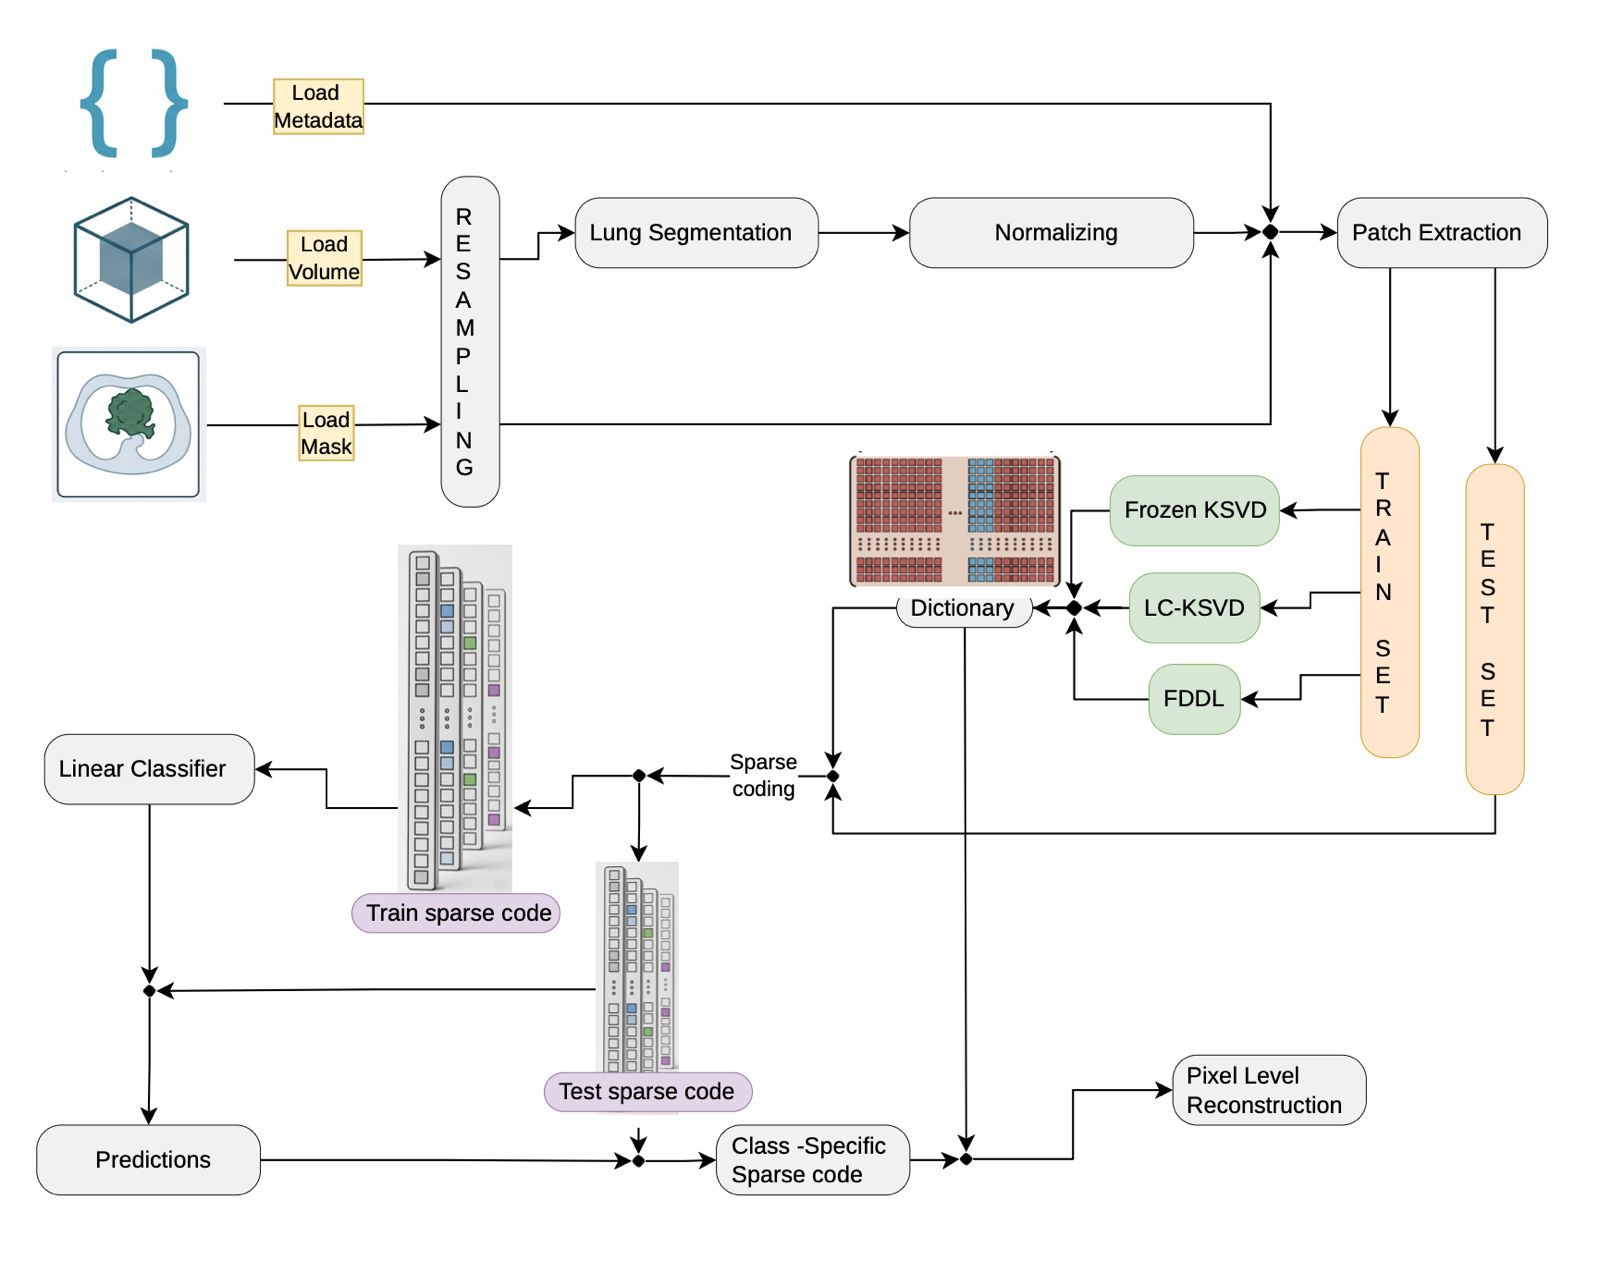
\includegraphics[width=\columnwidth]{OverallMethodologyDiagram.jpeg}
    \caption{Overview of the proposed framework.}
    \label{fig:methodology}
\end{figure}

Passing the whole volume to the model would include information on bones, soft tissue and background air which
risks letting the model pick up spurious patterns unrelated to lung pathology. Therefore, the lung region was isolated
using TotalSegmentator \cite{wasserthal2023totalsegmentator}. After lung segmentation, the voxel intensities were clipped to a fixed window of
$[-1000, 200] \text{HU}$. The lower bound corresponds to air, while $200 \text{HU}$ corresponds to the upper bound
derived using a histogram analysis of the dataset. Finally, Min-Max scaling to $[-1, 1]$ was used, prior to
extraction of fixed-size patches of normal lung parenchyma and lung abnormalities. Two target abnormalities were decided based
on expert Radiologist recommendation, sufficient representation within the dataset and clinical significance:
Ground-Glass Opacity (GGO), and Nodules/Masses. A patch size of $12 \times 12 \times 6$ is selected by considering
the average size of small nodules, the size of the dictionary, loss of context, and dataset variability. Furthermore, since
abnormalities are irregularly shaped, a maximum of 50\% of the voxels in a patch were allowed to be non-lesion.
A similar approach was used for healthy tissue, where a maximum of 50\% of the voxels in a patch were allowed to be
background to avoid patches sampled completely from outside the lung parenchyma. Each extracted patch is subsequently
flattened into a vector representation $\mathbf{y} \in \mathbb{R}^{n}$, where $n = 12 \times 12 \times 6$ is the number
of voxels, before being handed to the dictionary learning algorithms.

% Figure 2 shows the patch extraction pipeline.

% \begin{figure}[htbp]
%     \centering
%     \includegraphics[width=\columnwidth]{PatchExtraction.png}
%     \caption{Patch extraction pipeline.}
%     \label{fig:patch_extraction}
% \end{figure}

The extracted patches are divided to train and test splits, and four Dictionary Learning algorithms: K-SVD \cite{aharon2006ksvd},
LC-KSVD \cite{jiang2013lcksvd}, FDDL \cite{yang2011fddl} and Frozen Dictionary Learning \cite{carroll2017frozen}, are trained.
% The extracted patches are divided to train and test splits, and four Dictionary Learning algorithms: K-SVD,
% LC-KSVD, FDDL and Frozen Dictionary Learning, are trained.
For K-SVD and Frozen dictionary learning, the overcomplete dictionary $\mathbf{D} \in \mathbb{R}^{n \times K}$ is
formed by concatenating per-class sub-dictionaries,

\begin{equation}
    \mathbf{D} = \left[ \mathbf{D}_1 \,\middle|\, \mathbf{D}_2 \,\middle|\, \cdots \,\middle|\, \mathbf{D}_C \right], \qquad
    \mathbf{D}_c \in \mathbb{R}^{n \times K_c},
    \label{eq:dict_concat}
\end{equation}

where $C=3$ is the number of classes, $\mathbf{D}_c$ is the sub-dictionary associated with class $c$, $K_c = 3n$
is the number of atoms per class, and $K = \sum_{c=1}^{C} K_c$ is the total number of atoms. Specifically in Frozen dictionary learning,
abnormality sub-dictionaries are trained by keeping the normal lung parenchyma dictionary frozen.

For LC-KSVD and FDDL, $\mathbf{D}$ is learned jointly across all classes, with class structure encoded through a
label-consistency term or Fischer criterion. In each approach, the dictionary is made overcomplete
by setting the number of atoms to be 3 times the number of voxels in a patch, and the sparsity constraint
(maximum number of non-zero coefficients) $T = 10$ . The algorithms were implemented
in Python and released as an open-source PyPI package: \url{https://pypi.org/project/reppi/}.
Figure \ref{fig:ksvd_atoms} shows a visualization of the learned atoms from the K-SVD dictionary.

\begin{figure}
    \centering
    \includegraphics[width=\columnwidth]{atom_grid_normal_ggo_nodule.png}
    \caption{Visualization of learned atoms for each class.}
    \label{fig:ksvd_atoms}
\end{figure}

After training the dictionaries, the patches in the train split are re-encoded against each dictionary to produce a sparse code
for each patch. Given $\mathbf{D}$, a patch $\mathbf{y}$ is encoded by solving the sparsity-constrained least-squares problem

\begin{equation}
    \hat{\mathbf{x}} = \operatorname*{arg\,min}_{\mathbf{x} \in \mathbb{R}^{K}} \; \lVert \mathbf{y} - \mathbf{D}\mathbf{x} \rVert_2^2
    \quad \text{s.t.} \quad \lVert \mathbf{x} \rVert_0 \leq T,
    \label{eq:sparse_coding}
\end{equation}

where $\hat{\mathbf{x}} \in \mathbb{R}^{K}$ is the resulting sparse code.
A linear SVM model trains on these sparse codes and their corresponding labels. During inference,
the test patches are encoded against the learned dictionaries using Eq. \ref{eq:sparse_coding} to produce sparse codes,
which are then passed to the trained SVM classifier $f$ to predict the class label:

\begin{equation}
    \hat{c} = f(\hat{\mathbf{x}}), \qquad \hat{c} \in \{1, \dots, C\}.
    \label{eq:svm_predict}
\end{equation}

To localize the specific voxels in an abnormality patch, only the atoms corresponding to the predicted class are used,
while the remaining atoms are set to zero. We define a binary masking vector $\mathbf{m}_{\hat{c}} \in \{0,1\}^{K}$ that
retains only the coefficients belonging to the predicted class's atom index set $\mathcal{I}_{\hat{c}} \subset \{1, \dots, K\}$:

\begin{equation}
    \left(\mathbf{m}_{\hat{c}}\right)_k =
    \begin{cases}
        1, & k \in \mathcal{I}_{\hat{c}} \\
        0, & k \notin \mathcal{I}_{\hat{c}}
    \end{cases}
    \label{eq:mask}
\end{equation}

The masked sparse code is then $\tilde{\mathbf{x}} = \mathbf{m}_{\hat{c}} \odot \hat{\mathbf{x}}$.
The class-conditional reconstruction of the patch is given by

\begin{equation}
    \hat{\mathbf{y}}_{\hat{c}} = \mathbf{D}\tilde{\mathbf{x}} = \mathbf{D}_{\hat{c}}\,\hat{\mathbf{x}}_{\hat{c}},
    \label{eq:reconstruction}
\end{equation}

where $\hat{\mathbf{x}}_{\hat{c}} \in \mathbb{R}^{K_{\hat{c}}}$ denotes the sub-vector of $\hat{\mathbf{x}}$ restricted to
$\mathcal{I}_{\hat{c}}$. Eq. \ref{eq:reconstruction} isolates the contribution of only the predicted class's atoms,
suppressing the influence of atoms belonging to other classes and thereby localizing the reconstructed signal to the
voxels most consistent with the predicted abnormality. Figure \ref{fig:nodule_reconstruction} shows the final
reconstruction of a nodule using this technique.

\begin{figure}
    \centering
    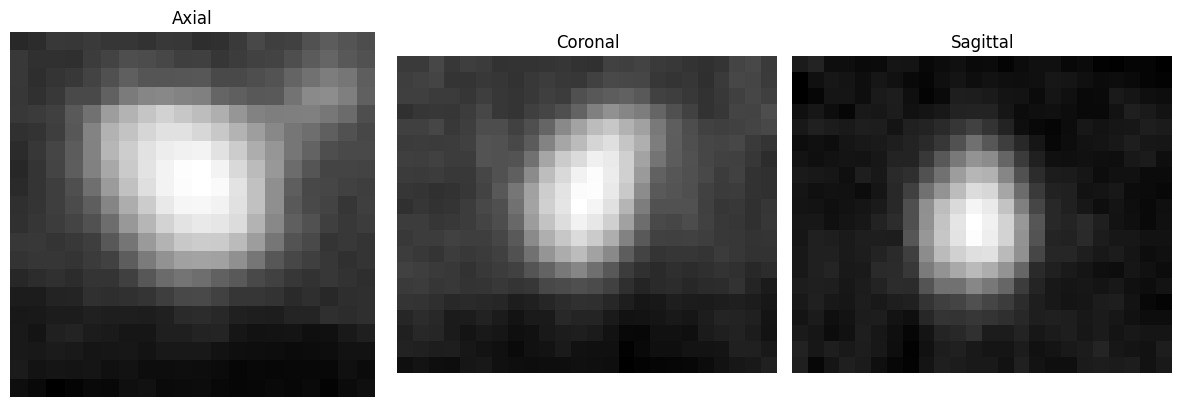
\includegraphics[width=\columnwidth]{NoduleReconstruction.jpeg}
    \caption{Reconstruction of a nodule using a learned dictionary.}
    \label{fig:nodule_reconstruction}
\end{figure}

\section{Evaluation Framework}
\label{sec:eval}

The 11 models compared in this study cover a range of approaches spanning sparse dictionary learning, dense voxel-wise
segmentation, and promptable foundation models. Their outputs at the end of a forward pass range from a calibrated
probability, to a bare class label, to a folder of binary volumes. To design an evaluation framework, all of these outputs have
to be pushed through one common representation. The shared framework consists of three components: a Runner, Core, and
Adapter. The Adapter translates each model's native output into a common case schema without performing any computations,
making it easy to add new models by implementing only this conversion step. The Core is a model-agnostic library
containing consistent metric definitions for classification, localization, and explainability, operating exclusively on the
common schema so that all models are evaluated using identical calculations. The Runner connects the two by selecting the
appropriate Adapter and Core metrics for a given model and evaluation axis, then producing summary and per-case results.
The framework is used to evaluate the dictionary learning models, three machine learning baselines: Logistic Regression,
Linear SVM, and XGBoost, and four SotA deep learning models: CT-CLIP \cite{hamamci2024ctclip}, Merlin \cite{Blankemeier2026},
BiomedParse \cite{zhao2025foundation}, and nnU-Net \cite{isensee2021nnu}.
The framework is deployed as a public benchmark on Huggingface: \url{https://huggingface.co/spaces/Gotech/cad-benchmark}.

\begin{table*}[t]
    \centering
    \caption{Summary of results across all models and evaluation axes.}
    \label{tab:results-summary}
    \renewcommand{\arraystretch}{1.5}
    \resizebox{0.9\textwidth}{!}{
        \begin{tabular}{llcccccccccc}
            \hline
            \textbf{Model Type} & \textbf{Model} &
            \multicolumn{5}{c}{\textbf{Classification}} &
            \multicolumn{3}{c}{\textbf{Segmentation}} &
            \multicolumn{2}{c}{\textbf{Explainability}} \\
            \cline{3-7}
            \cline{8-10}
            \cline{11-12}
            & &
            \textbf{Accuracy} & \textbf{Precision} & \textbf{Recall} &
            \textbf{F1} & \textbf{AU-ROC} &
            \textbf{Dice} & \textbf{Hit Rate} & \textbf{IoU} &
            \textbf{PG Acc.} & \textbf{EIM} \\
            \hline

            \multirow{4}{*}{\makecell{Dictionary\\Learning}}

            & LC-KSVD
            & 0.885 & 0.896 & 0.885 & 0.888 & 0.97
            & 0.010 & 0.200 & 0.005 & -- & -- \\

            & K-SVD
            & 0.664 & 0.653 & 0.630 & 0.631 & 0.72
            & 0.004 & 0.080 & 0.002 & -- & -- \\

            & FDDL
            & 0.766 & 0.759 & 0.724 & 0.737 & 0.83
            & 0.006 & 0.120 & 0.003 & -- & -- \\

            & Frozen DL
            & 0.824 & 0.824 & 0.784 & 0.801 & 0.89
            & 0.008 & 0.160 & 0.004 & -- & -- \\

            \hline

            \multirow{3}{*}{\makecell{Machine\\Learning}}
            & Linear SVM
            & 0.592 & 0.580 & 0.580 & 0.580 & 0.65
            & -- & -- & -- & -- & -- \\

            & Log. Regression
            & 0.554 & 0.539 & 0.540 & 0.539 & 0.62
            & -- & -- & -- & -- & -- \\

            & XGBoost
            & 0.524 & 0.510 & 0.509 & 0.510 & 0.57
            & -- & -- & -- & -- & -- \\

            \hline

            \multirow{4}{*}{\makecell{Deep\\Learning}}
            & CT-CLIP
            & 0.600 & 0.594 & 0.587 & 0.590 & 0.68
            & -- & -- & -- & 0.03 & 0.14 \\

            & Merlin
            & 0.950 & 0.950 & 0.948 & 0.949 & 0.90
            & -- & -- & -- & 0.06 & 0.09 \\

            & BiomedParse
            & -- & -- & -- & -- & --
            & 0.27 & 0.64 & 0.63 & 0.93 & 0.84 \\

            & nnU-Net
            & -- & -- & -- & -- & --
            & 0.10 & 0.14 & 0.05 & 0.08 & 0.12 \\

            \hline
        \end{tabular}
    }
\end{table*}

\section{Results and Discussion}
\label{sec:results}

Table \ref{tab:results-summary} provides a summary of the results across all models and evaluation axes.
LC-KSVD outperformed all other dictionary learning models, reaching 88.5\% patch accuracy.
Patch-level accuracy did not transfer to localisation for any dictionary learning method,
a gap driven by the extreme size imbalance between lesions and full volumes rather than by
the sparse codes themselves. Dictionary learning trails SotA deep learning substantially on raw performance, confirming a
interpretability-performance trade-off. Merlin achieved the highest classification accuracy of 95\%, while
BiomedParse achieved the highest segmentation hit rate of 65\%.

% To start a new column (but not a new page) and help balance the last-page
% column length use \vfill\pagebreak.
% -------------------------------------------------------------------------
\vfill
\pagebreak

% References should be produced using the bibtex program from suitable
% BiBTeX files (here: strings, refs, manuals). The IEEEbib.bst bibliography
% style file from IEEE produces unsorted bibliography list.
% ------------------------------------------------------------------------- 
\bibliographystyle{IEEEbib}
\bibliography{strings,refs}

\end{document}
